\documentclass{article} % For LaTeX2e
\usepackage{nips14submit_e,times}
\usepackage{amsmath}
\usepackage{amsthm}
\usepackage{amssymb}
\usepackage{mathtools}
\usepackage{hyperref}
\usepackage{url}
\usepackage{algorithm}
\usepackage[noend]{algpseudocode}
%\documentstyle[nips14submit_09,times,art10]{article} % For LaTeX 2.09

\usepackage{bbm}
\usepackage{graphicx}
\usepackage{caption}
\usepackage{subcaption}
\usepackage{MnSymbol}

\def\eQb#1\eQe{\begin{eqnarray*}#1\end{eqnarray*}}
\def\eQnb#1\eQne{\begin{eqnarray}#1\end{eqnarray}}
\providecommand{\e}[1]{\ensuremath{\times 10^{#1}}}
\providecommand{\pb}[0]{\pagebreak}
\DeclarePairedDelimiter\ceil{\lceil}{\rceil}
\DeclarePairedDelimiter\floor{\lfloor}{\rfloor}

\newcommand{\E}{\mathrm{E}}
\newcommand{\Var}{\mathrm{Var}}
\newcommand{\Cov}{\mathrm{Cov}}
\newcommand\eqD{\stackrel{\mathclap{\normalfont\mbox{d}}}{=}}

\def\Qb#1\Qe{\begin{question}#1\end{question}}
\def\Sb#1\Se{\begin{solution}#1\end{solution}}

\newenvironment{claim}[1]{\par\noindent\underline{Claim:}\space#1}{}
\newtheoremstyle{quest}{\topsep}{\topsep}{}{}{\bfseries}{}{ }{\thmname{#1}\thmnote{ #3}.}
\theoremstyle{quest}
\newtheorem*{definition}{Definition}
\newtheorem*{theorem}{Theorem}
\newtheorem*{lemma}{Lemma}
\newtheorem*{question}{Question}
\newtheorem*{preposition}{Preposition}
\newtheorem*{exercise}{Exercise}
\newtheorem*{challengeproblem}{Challenge Problem}
\newtheorem*{solution}{Solution}
\newtheorem*{remark}{Remark}
\usepackage{verbatimbox}
\usepackage{listings}
\usepackage{mathrsfs}
\title{ProbLimI: \\
Problem Set XIII}


\author{
Youngduck Choi \\
CIMS \\
New York University\\
\texttt{yc1104@nyu.edu} \\
}


% The \author macro works with any number of authors. There are two commands
% used to separate the names and addresses of multiple authors: \And and \AND.
%
% Using \And between authors leaves it to \LaTeX{} to determine where to break
% the lines. Using \AND forces a linebreak at that point. So, if \LaTeX{}
% puts 3 of 4 authors names on the first line, and the last on the second
% line, try using \AND instead of \And before the third author name.

\newcommand{\fix}{\marginpar{FIX}}
\newcommand{\new}{\marginpar{NEW}}

\nipsfinalcopy % Uncomment for camera-ready version

\begin{document}


\maketitle

\begin{abstract}
This work contains solutions to the exercises of the problem set IX. The
chosen problems are 2,3 and 4.
\end{abstract}

\bigskip

\begin{question}[1]
\hfill
\begin{figure}[h!]
  \centering
    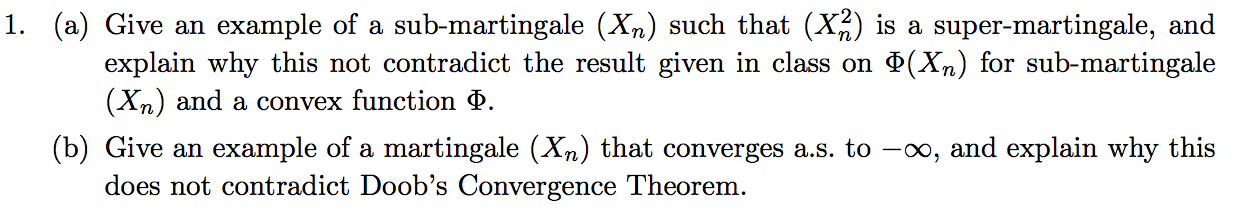
\includegraphics[width=0.7\textwidth]{problim-e13-p1.png}
\end{figure}
\end{question}
\begin{solution} \hfill \\
\textbf{(a)} Let
$X_n = 0$ for each $n \geq 1$, then ${X_n}^2 = 0$ for each $n \geq 1$.
It follows that $\{X_n\}$ is a sub-martingale, and $\{X_n^{2}\}$ is a super-martingale
because they are both martingales trivially, as 
\eQb
\mathbb{E}[X_n | \mathscr{F}_{n-1}] = X_n = X_{n-1} = 0
\eQe
and
\eQb
\mathbb{E}[X_n^2 | \mathscr{F}_{n-1}] = X_n^2 = X_{n-1}^2 = 0
\eQe
for each $n \geq 1$. This does not contradict the given fact about the convex function,
as $\{X_n^2\}$ is a sub-martingale as well, by being a martingale.

\bigskip

\textbf{(b)} Let $\{ X_n \}$ i.i.d random variables be defined by
\eQb
\mathbb{P}(X_n = -1) = 1  - \dfrac{1}{2^n} \>\>\> \text{and} \>\>\>
\mathbb{P}(X_n = 2^{n} - 1) = \dfrac{1}{2^n} 
\eQe 
for each $n \geq 1$. Then,
\eQb
\mathbb{E}[X_n] = 0 
\eQe
for each $n \geq 1$, so $\{S_n = \sum_{k=1}^{n} X_k\}$ 
is a martingale with respect to the
canonical filteration. Observe that
\eQb
\sum_{n=1}^{\infty} \mathbb{P}( X_n > -1  ) = 
\sum_{n=1}^{\infty} \dfrac{1}{2^n} < \infty
\eQe
By Borel-Cantelli,
\eQb
\mathbb{P}(X_n > -1 \>\> i.o. ) = 0 
\eQe
and hence
\eQb
\mathbb{P}(X_n \leq -1  \>\> a.a. ) = 1. 
\eQe
Therefore, $S_n \to -\infty$ almost surely and we are done. This 
does not violate the Martingale convergence theorem, as 
$\sup_n \mathbb{E}[|S_n|]$ is not bounded. 

\bigskip

\end{solution}

\newpage

\begin{question}[3]
\hfill
\begin{figure}[h!]
  \centering
    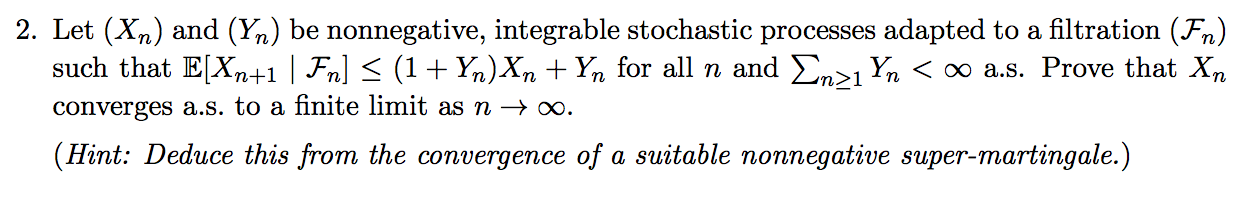
\includegraphics[width=0.7\textwidth]{problim-e13-p2.png}
\end{figure}
\end{question}
\begin{solution} \hfill \\
\end{solution}

\newpage

\begin{question}[4]
\hfill
\begin{figure}[h!]
  \centering
    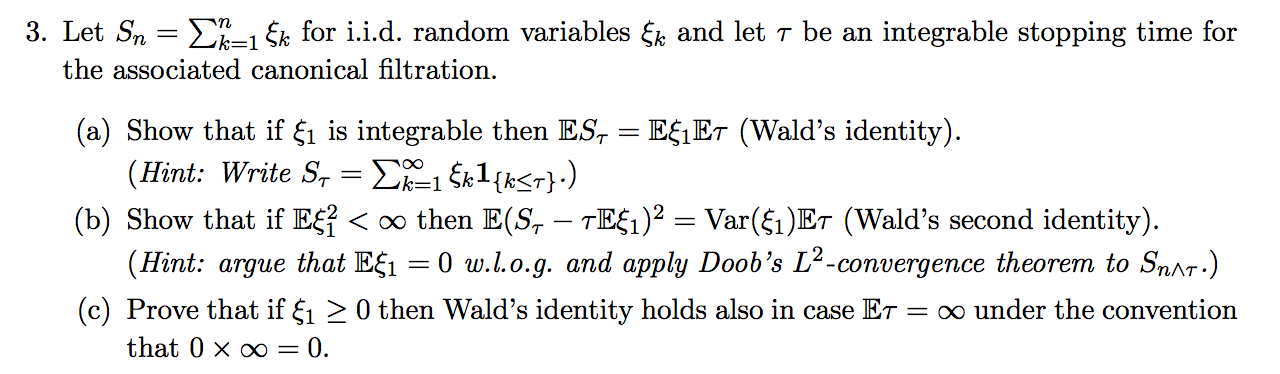
\includegraphics[width=0.7\textwidth]{problim-e13-p3.png}
\end{figure}
\end{question}
\begin{solution} \hfill \\
\textbf{(a)} Observe that 
\eQb
\xi_i \text{ and } 1_{\{i \leq \tau\}} \text{ are independent} 
\eQe
for each $i \geq 1$. Now, we first prove for the case when $\xi_i \geq 0$ for all $i 
\geq 1$. 
\eQnb
\mathbb{E}[S_{\tau}] &=& \mathbb{E}[\xi_1 + ... + \xi_{\tau}] = 
\mathbb{E}[\sum_{i=1}^{\infty} \xi_i 1_{\{i \leq \tau\}}]  \nonumber \\
&=& \sum_{i=1}^{\infty} \mathbb{E}[\xi_i 1_{\{i \leq \tau \}}] 
= \sum_{i=1}^{\infty} \mathbb{E}[\xi_i] \mathbb{E}[1_{\{i \leq \tau\}}] 
\label{eq:4.1} \\
&=& \mathbb{E}[\xi_1] \sum_{i=1}^{\infty}\mathbb{P}(i \leq \tau) = 
\mathbb{E}[\xi_1] \mathbb{E}[\tau] \label{eq:4.2}
\eQne
where ~\eqref{eq:4.1} holds by MCT (or Tonelli) and independence,
and ~\eqref{eq:4.2} holds as $\tau$
being a non-negative integer valued random variable. Now consider a general $\{\xi_i\}$.
From the above, 
\eQb
\mathbb{E}[\sum_{i=1}^{\infty} |\xi_i| 1_{\{i\leq \tau\}}] =  
\mathbb{E}[|\xi_1|] \mathbb{E}[\tau] < \infty. 
\eQe 
Therefore, by Fubini,
\eQb
\mathbb{E}[\xi_{\tau}] = 
\mathbb{E}[\sum_{i=1}^{\infty} \xi_i 1_{\{i \leq \tau\}}] &=&
\sum_{i=1}^{\infty} \mathbb{E}[\xi_i 1_{\{i \leq \tau\}}] = \mathbb{E}[\xi_1]
\mathbb{E}[\tau]. 
\eQe
\end{solution}

\end{document}
